\section{Data Transformation}
\begin{tcolorbox}[title=It's Also True of Data]
History is the transformation of tumultuous conquerors into silent footnotes. \\[-0.6cm]
\begin{flushright}
-- Paul Eldridge, American educator
\end{flushright}
\end{tcolorbox}
\noindent
This \textbf{crucial} last step is often neglected or omitted altogether. Various transformation methods are available, depending on the analysts' needs and data types, including: \begin{itemize}[noitemsep]
\item \textbf{standardization} and \textbf{unit conversion}, which put the dataset's variables on an equal footing -- a requirement for basic comparison tasks and more complicated problems of clustering and similarity matching;
\item \textbf{normalization}, which  attempts to force a variable into a normal distribution -- an assumption which must be met in order to use a number of traditional analysis methods, such as ANOVA or regression analysis, and 
\item \textbf{smoothing methods}, which help remove unwanted noise from the data, but at a price -- perhaps removing natural variance in the data. 
\end{itemize}
Another type of data transformation is pre-occupied with the concept of \textbf{dimensionality reduction}. There are many advantages to working with low-dimensional data \cite{DAL_FSDR}:
\begin{itemize}[noitemsep]
\item \textbf{visualization methods} of all kinds are available to extract and present insights out of such data;
\item high-dimensional datasets are subject to the so-called \textbf{curse of dimensionality}, which asserts (among other things) that multi-dimensional spaces are vast, and when the number of features
in a model increases, the number of observations required to maintain predictive
power also increases, but at a \textbf{substantially higher rate} (see Figure~\ref{fig:COD});
\item another consequence of the curse is that in high-dimension sets, all observations are roughly \textbf{dissimilar} to one another -- observations tend to be nearer the dataset's boundaries than they are to one another.  
\end{itemize}
\begin{figure*}[t]
\centering
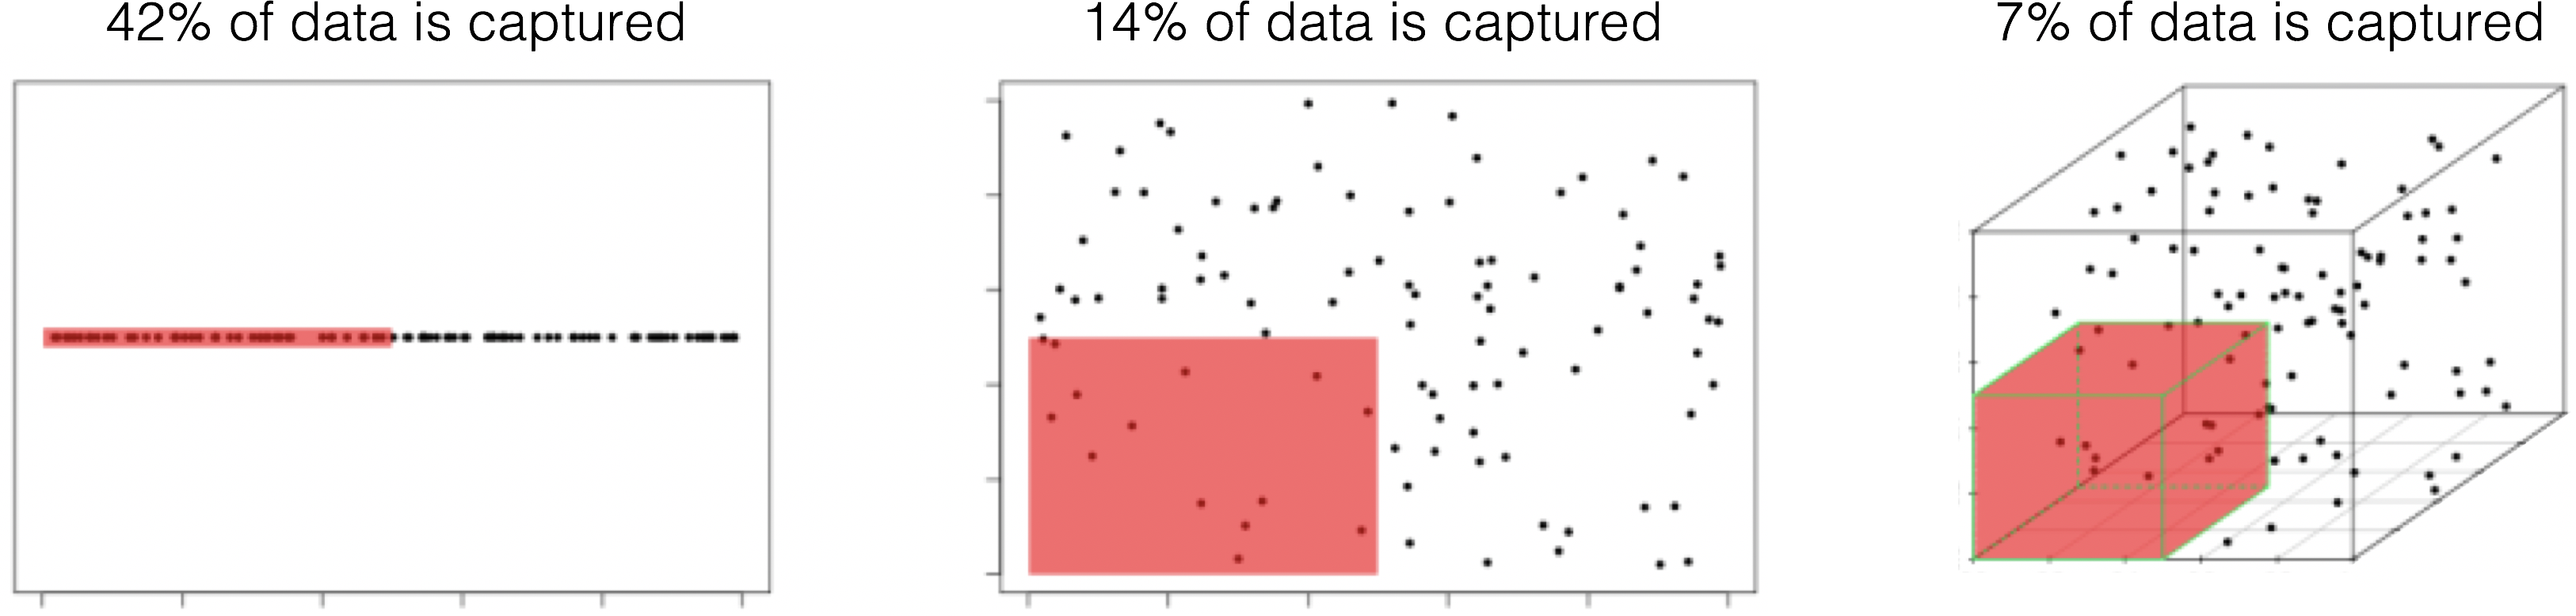
\includegraphics[width=\textwidth]{Images/COD.png}\caption[\small Illustration of the curse of dimensionality]{\small Illustration of the curse of dimensionality; $N=100$ observations are uniformly distributed on the unit hypercube $[0,1]^d$, $d=1, 2, 3$. The red regions represent the smaller hypercubes $[0,0.5]^d$, $d=1,2,3$. The percentage of captured datapoints is seen to decrease with an increase in $d$ \cite{DP_SS}.} \label{fig:COD}\hrule
\end{figure*}
Dimension reduction techniques such as \textbf{principal component analysis}, \textbf{independent component analysis}, and \textbf{factor analysis} (for numerical data), or \textbf{multiple correspondence analysis} (for categorical data) project multi-dimensional datasets onto low-dimensional but high information spaces (the so-called \textbf{Manifold Hypothesis}). Some information is necessarily lost in the process, but in many instances the drain can be kept under control and the gains made by working with smaller datasets can offset the losses of completeness \cite{DAL_FSDR}.
\subsection{Common Transformations} Models often require that certain data assumptions be met. For instance, ordinary least square regression assumes:
\begin{itemize}[noitemsep]
\item that the response variable is a \textbf{linear combination} of the predictors;
\item \textbf{constant} error variance; 
\item \textbf{uncorrelated residuals}, which may or may not be statistically independent;
\item etc.
\end{itemize}
In reality, it is rare that raw data  meets all these requirements, but that does not necessarily mean that we need to abandon the model -- an \textbf{invertible} sequence of data transformations may produce a derived data set which \textit{does} meet the requirements, allowing the consultant to draw conclusions about the original data. \par In the regression context, invertibility is guaranteed by \textbf{monotonic} transformations:  identity, logarithmic, square root, inverse (all members of the power transformations), exponential, etc. (illustrations are provided in Figure~\ref{fig:transforms}).
\begin{figure*}[t]
\centering
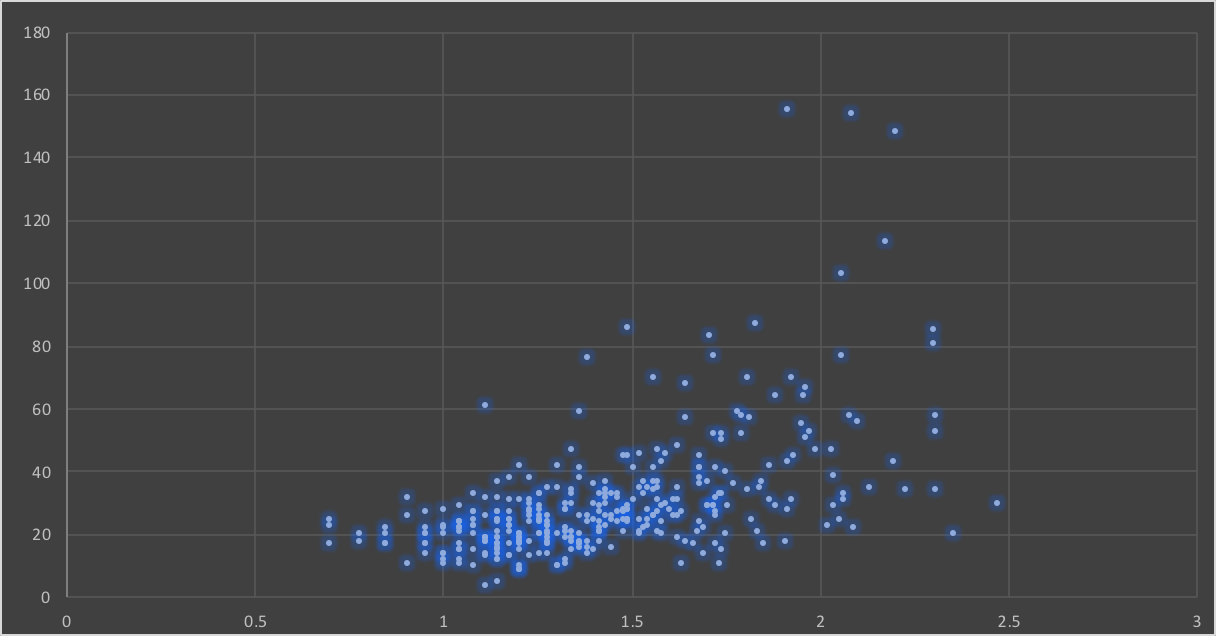
\includegraphics[width=0.48\textwidth]{Images/original_BUPA.png}
\quad
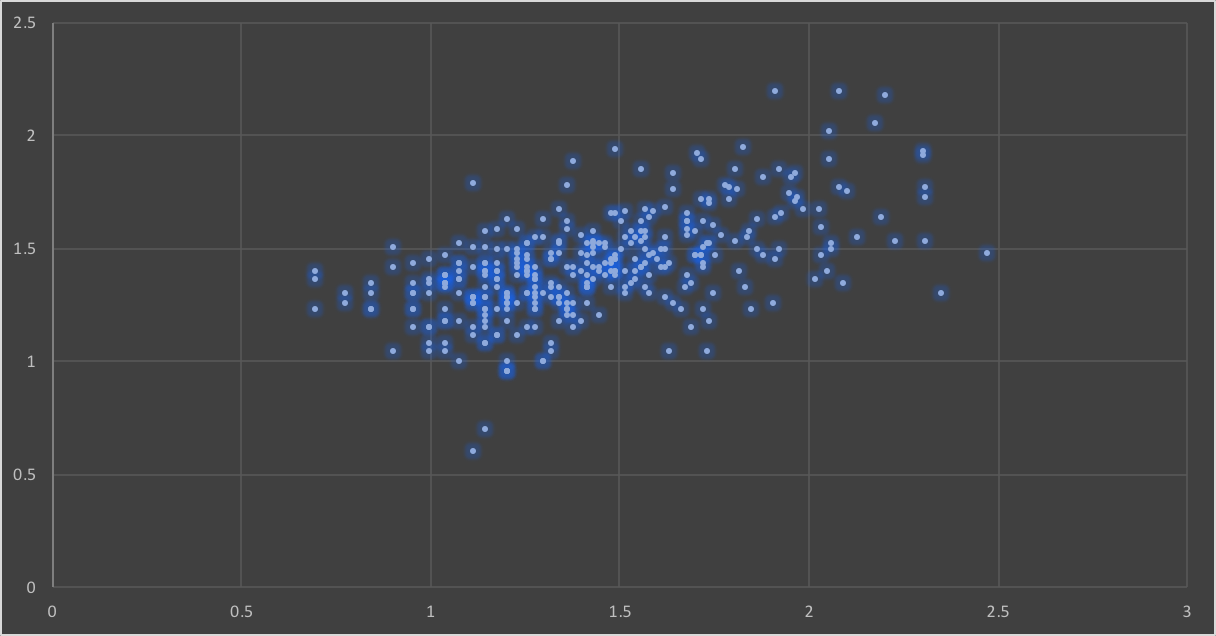
\includegraphics[width=0.48\textwidth]{Images/log.png} \\
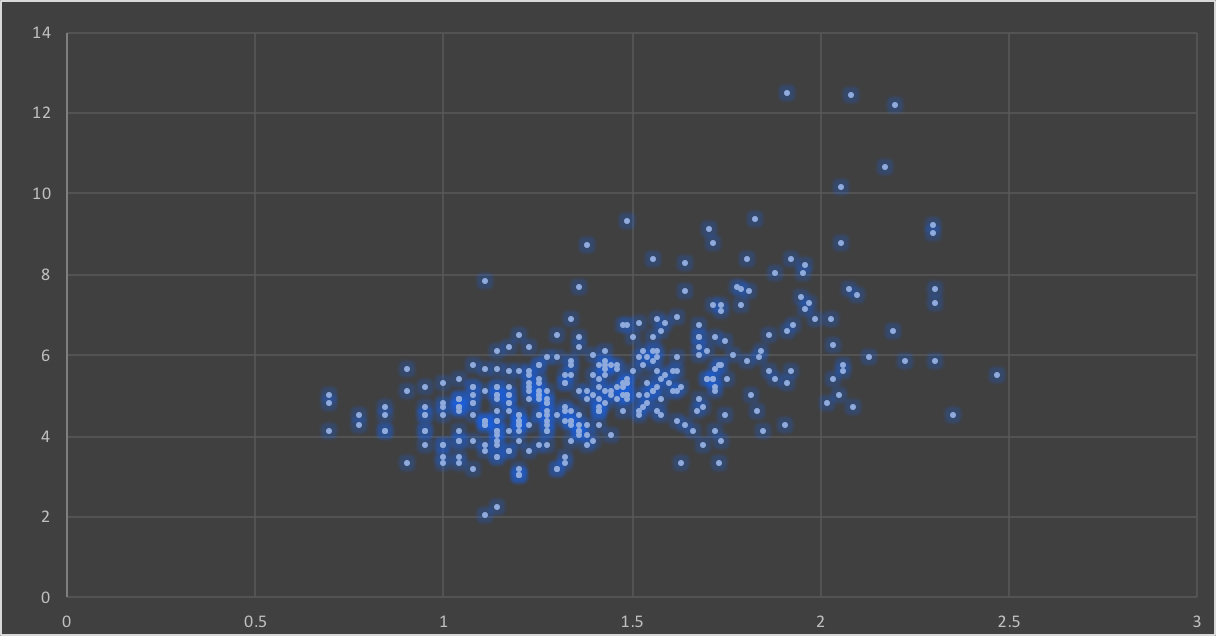
\includegraphics[width=0.48\textwidth]{Images/sqrt.png} 
\quad
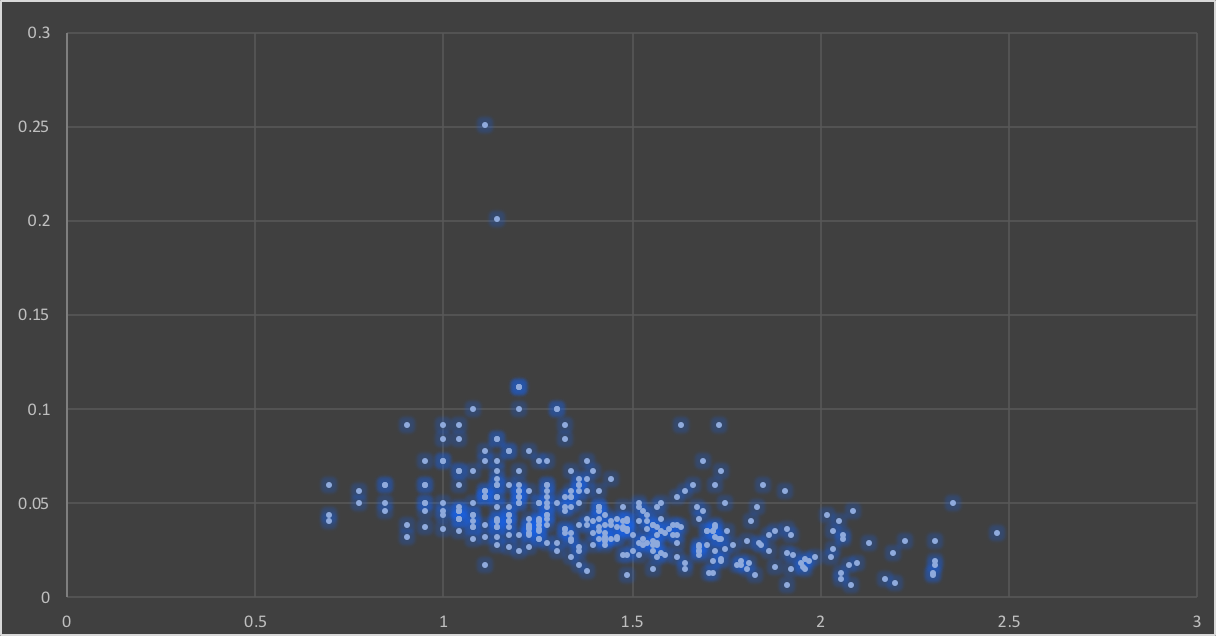
\includegraphics[width=0.48\textwidth]{Images/inverse.png} \\
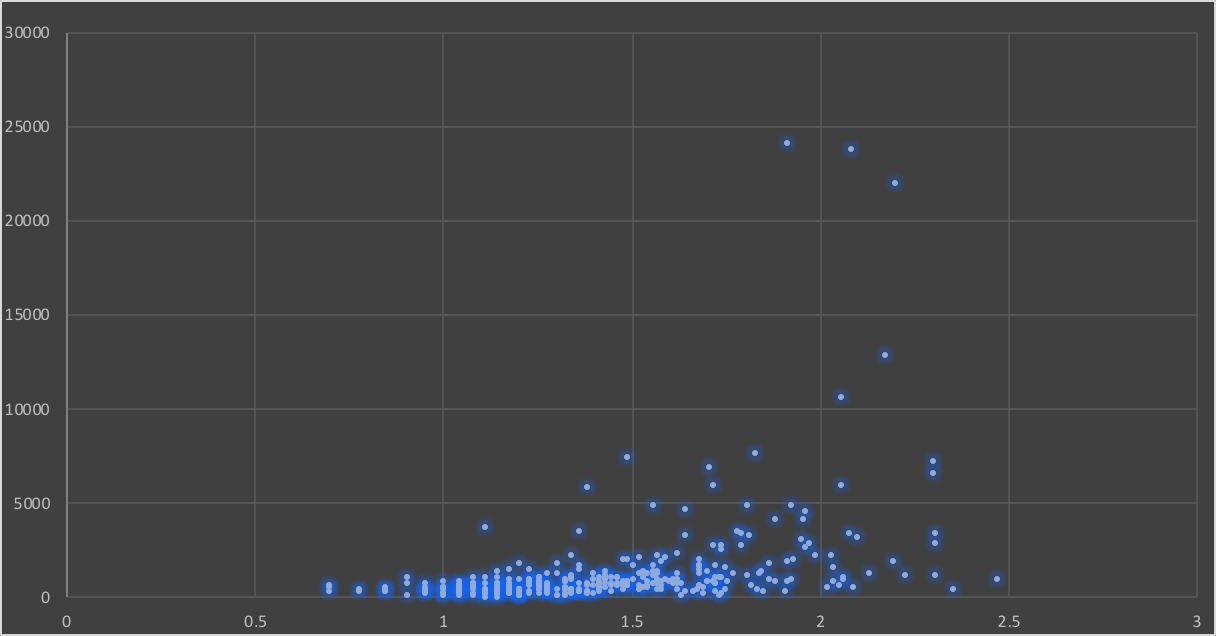
\includegraphics[width=0.48\textwidth]{Images/square.png} 
\quad
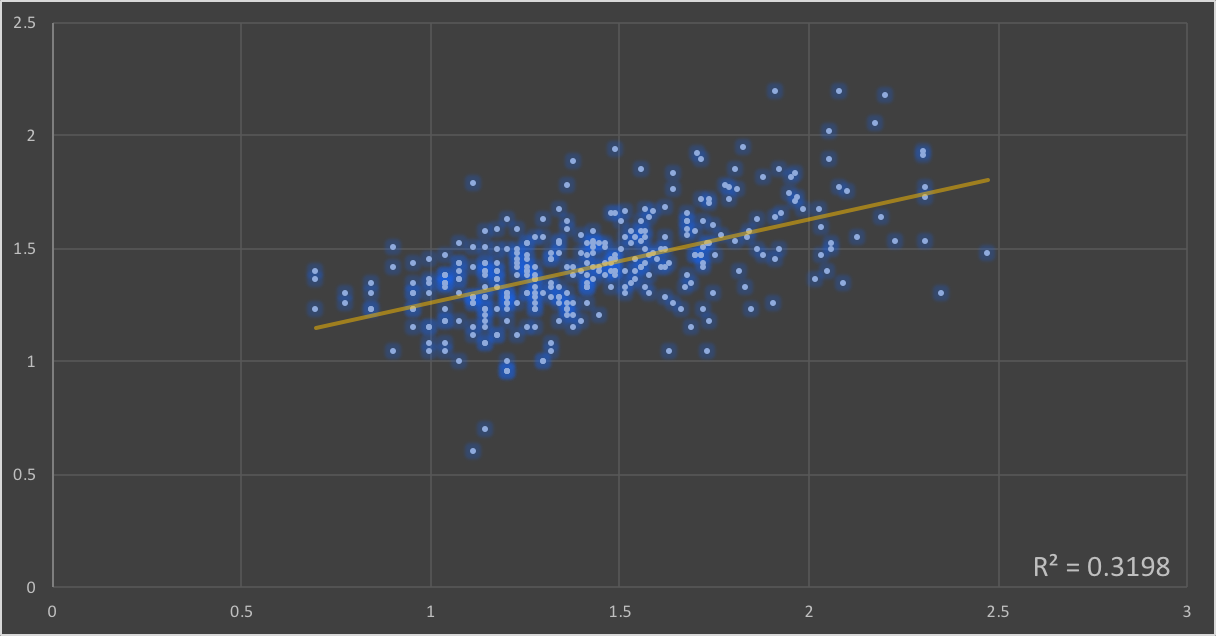
\includegraphics[width=0.48\textwidth]{Images/boxcox.png}
\caption[\small Examples of data transformations]{\small Examples of data transformations, for a subset of the BUPA liver dataset \cite{DP_BUPA}. From left to right, top to bottom: original data, $Y'=\log Y$, $Y'=\sqrt{Y}$, $Y'=\frac{1}{Y}$, $Y'=Y^2$, and Box-Cox best choice ($\approx$ log). }
\hrule\label{fig:transforms}
\end{figure*}
\par There are rules of thumb and best practices to transform data, but analysts and consultants should not discount the importance of exploring the data visually before making a choice. \newl Transformations on the predictors $X$ may be used to achieve the \textbf{linearity assumption}, but they usually come at a price -- correlations are not preserved by such transformations, for instance. Transformations on the target $Y$ can help with \textbf{non-normality} of residuals and \textbf{non-constant variance} of error terms. \par Note that transformations can be applied \textbf{both} to the target variable or the predictors: as an example, if the linear relationship between two variables $X$ and $Y$ is expressed as $Y=a+bX$, then a unit increase in $X$ is associated with an average of $b$ units in $Y$. \newl But a better fit might be afforded by either of $$\log Y = a+bX,\quad Y=a+b\log X,\quad \mbox{or}\quad  \log Y = a+b\log X,$$ for which:
\begin{itemize}[noitemsep]
\item a unit increase in $X$ is associated with an average $b\%$ increase in $Y$;
\item a $1\%$ increase in $X$ is associated with an average $0.01b$ unit increase in $Y$, and
\item a $1\%$ increase in $X$ is associated with a $b\%$ increase in $Y$, respectively. 
\end{itemize}
\subsection{Box-Cox Transformation} The choice of transformation is often as much of an art as it is a science. There is a common  framework, however, that provides the  optimal transformation, in a sense. Consider the task of predicting the target $Y$ with the help of the predictors $X_j$, $j=1,\ldots, p$. The usual model takes the form $$y_i=\sum_{j=1}^p\beta_jX_{x,i}+\varepsilon_i,\quad i=1,\ldots, n.$$ If the residuals are skewed, or their variance is not constant, or the trend itself does not appear to be linear, a power transformation might be preferable, but if so,  which one? \newl The \textbf{Box-Cox transformation} $y_i\mapsto y'_i(\lambda)$, $y_i>0$ is defined by  $$y'_i(\lambda)=\begin{cases}(y_1 \ldots   y_n)^{1/n}\ln y_i, \text{if }\lambda=0 \\ 
\frac{y_i^{\lambda}-1}{\lambda}(y_1 \ldots   y_n)^{\frac{1-\lambda}{n}}, \text{if }\lambda\neq 0
\end{cases};$$
variants allow for the inclusion of a shit parameter $\alpha>0$, which extends the transformation to $y_i>-\alpha$. The \textbf{suggested} choice of $\lambda$ is the value that maximises the log-likelihood $$\mathcal{L}=-\frac{n}{2}\log\left(\frac{2\pi\hat{\sigma}^2}{(y_1 \ldots   y_n)^{2(\lambda-1)/n}}+1\right).$$
There might be theoretical rationales which favour a particular choice of $\lambda$ -- these are not to be ignored. It is also important to produce a residual analysis, as the best Box-Cox choice does not necessarily meet all the least squares assumptions. \newl Finally, it is important to remember that the resulting parameters have the least squares property \textbf{only with respect to the transformed data points}. 
\subsection{Scaling} Numeric variables may have different scales (weights and heights, for instance). Since the variance of a large-range variable is typically greater than that of a small-range variable, leaving the data \textbf{unscaled} may introduce biases, especially when using unsupervised methods.\par  It could also be the case that it is the relative positions (or rankings) which is of importance, in which case it could become important to look at relative distances between levels: 
\begin{itemize}[noitemsep]
\item \textbf{standardisation} creates a variable with mean 0 and standard deviations 1: $$Y_i=\frac{X_i-\overline{X}}{s_X};$$
\item \textbf{normalization} creates a variable in the range [0,1]: $$Y_i=\frac{X_i-\min\{X_k\}}{\max \{X_k\}- \min \{X_k\}}.$$
\end{itemize}
These are not the only options. Different schemes can lead to different outputs. 
\subsection{Discretizing} To reduce computational complexity, a numeric variable may need to be replaced with an \textbf{ordinal} variable (\textit{height} values could be replaced by the qualitative ``\textit{short}'', ``\textit{average}'', and ``\textit{tall}'', for instance. \par Of course, what these terms represent depend on the context: Canadian short and Bolivian tall may be fairly commensurate, to revisit the example at the start of the preceding section.  \newpage\noindent It is far from obvious how to  determine the bins' limits  -- \textbf{domain expertise} can help, but it could introduce unconscious bias to the analyses. In the absence of such expertise, limits can be set so that either the bins each: 
\begin{itemize}[noitemsep]
\item contain the same \textbf{number of observations};
\item have the same \textbf{width}, or 
\item the performance of some modeling tool is maximised. 
\end{itemize}
Again, various choices may lead to different outputs. 
\subsection{Creating Variables} Finally, it is possible that new variables may need to be introduced (in contrast with dimensionality reduction). These new variables may arise
\begin{itemize}[noitemsep]
\item as \textbf{functional relationships} of some subset of available features (introducing powers of a feature, or principal components, say);
\item because modeling tool may require \textbf{independence of observations} or \textbf{independence of features} (in order to remove multicolinearity, for instance), or 
\item to simplify the analysis by looking at \textbf{aggregated summaries} (often used in text analysis).
\end{itemize}
There is no limit to the number of new variables that can be added to a dataset -- but consultants should strive for \textbf{relevant additions}.